% This is the Reed College LaTeX thesis template. Most of the work
% for the document class was done by Sam Noble (SN), as well as this
% template. Later comments etc. by Ben Salzberg (BTS). Additional
% restructuring and APA support by Jess Youngberg (JY).
% Your comments and suggestions are more than welcome; please email
% them to cus@reed.edu
%
% See https://www.reed.edu/cis/help/LaTeX/index.html for help. There are a
% great bunch of help pages there, with notes on
% getting started, bibtex, etc. Go there and read it if you're not
% already familiar with LaTeX.
%
% Any line that starts with a percent symbol is a comment.
% They won't show up in the document, and are useful for notes
% to yourself and explaining commands.
% Commenting also removes a line from the document;
% very handy for troubleshooting problems. -BTS

% As far as I know, this follows the requirements laid out in
% the 2002-2003 Senior Handbook. Ask a librarian to check the
% document before binding. -SN

%%
%% Preamble
%%
\pdfobjcompresslevel 0 % pour être pris en charge par la plateforme d'archivage du CINES
% voir https://facile.cines.fr#latex
% \documentclass{<something>} must begin each LaTeX document
\documentclass[12pt,a4paper]{reedthesis}
% Packages are extensions to the basic LaTeX functions. Whatever you
% want to typeset, there is probably a package out there for it.
% Chemistry (chemtex), screenplays, you name it.
% Check out CTAN to see: https://www.ctan.org/
%%
\usepackage{graphicx,latexsym}
\usepackage{amsmath,amssymb,amsthm}
\usepackage{amsfonts}
\usepackage{longtable,booktabs,setspace}
% \usepackage{chemarr} %% Useful for one reaction arrow, useless if you're not a chem major
\usepackage[hyphens]{url}
% Added by CII
\usepackage{lmodern}
\usepackage{float}
\floatplacement{figure}{H}
% End of CII addition
\usepackage{rotating}
\usepackage{tcolorbox} %New Kim
\usepackage[utf8]{inputenc}
\usepackage[T1]{fontenc}
\usepackage{fancyhdr}
\usepackage{xcolor}
\definecolor{Prune}{RGB}{99,0,60}
\definecolor{Pink}{RGB}{233,200,225} %new Kim
\usepackage{mdframed}
\usepackage{multirow} %% Pour mettre un texte sur plusieurs rangées
\usepackage{multicol} %% Pour mettre un texte sur plusieurs colonnes
\usepackage{scrextend} %Forcer la 4eme  de couverture en page pair
\usepackage{tikz}
\usepackage[absolute]{textpos}
\usepackage{colortbl}
\usepackage{array}
%\RequirePackage{geometry}% That nicely create a one-page template
%\geometry{textheight=100ex,textwidth=40em,top=30pt,headheight=30pt,headsep=30pt,inner=80pt}
\usepackage{geometry}
\usepackage{hyperref}
%\usepackage[pagebackref=true]{hyperref}

% Next line commented out by CII
%%% \usepackage{natbib}
% Comment out the natbib line above and uncomment the following two lines to use the new
% biblatex-chicago style, for Chicago A. Also make some changes at the end where the
% bibliography is included.
%\usepackage{biblatex-chicago}
%\bibliography{thesis}

% New Kim
\newenvironment{note}{
{\setstretch{0.5} %new pour changer le linespace des sources
\vspace{-0.5cm}
\footnotesize
}
}

% new tcolorbox environment Kim
\newtcolorbox{encadre}{
  colback=Pink,
  colframe=Prune,
  coltext=Prune,
  boxsep=5pt,
  arc=4pt
}

% Enlever les sous-titres des annexes dans le toc Kim
% \newcommand{\stoptocwriting}{%
%   \addtocontents{toc}{\protect\setcounter{tocdepth}{-5}}}
% \newcommand{\resumetocwriting}{%
%   \addtocontents{toc}{\protect\setcounter{tocdepth}{\arabic{tocdepth}}}}
\usepackage{etoolbox}
\appto\appendix{\addtocontents{toc}{\protect\setcounter{tocdepth}{0}}}
% reinstate the correct level for list of tables and figures
\appto\listoffigures{\addtocontents{lof}{\protect\setcounter{tocdepth}{1}}}
\appto\listoftables{\addtocontents{lot}{\protect\setcounter{tocdepth}{1}}}

\usepackage[french]{babel}


  
% Added by CII (Thanks, Hadley!)
% Use ref for internal links
%\renewcommand{\hyperref}[2][???]{\autoref{#1}}
\def\chapterautorefname{Chapitre}
\def\sectionautorefname{Section}
\def\subsectionautorefname{Sous-section}
% End of CII addition

% Added by CII
\usepackage{caption}
\captionsetup{width=5in}
% End of CII addition

% \usepackage{times} % other fonts are available like times, bookman, charter, palatino

% Syntax highlighting #22
$if(highlighting-macros)$
  $highlighting-macros$
$endif$


% Added by CII
%%% Copied from knitr
%% maxwidth is the original width if it's less than linewidth
%% otherwise use linewidth (to make sure the graphics do not exceed the margin)
\makeatletter
\def\maxwidth{ %
  \ifdim\Gin@nat@width>\linewidth
    \linewidth
  \else
    \Gin@nat@width
  \fi
}
\makeatother

%Added by @MyKo101, code provided by @GerbrichFerdinands
$if(csl-refs)$
\newlength{\cslhangindent}
\setlength{\cslhangindent}{1.5em}
\newenvironment{CSLReferences}%
  {$if(csl-hanging-indent)$\setlength{\parindent}{0pt}%
  \everypar{\setlength{\hangindent}{\cslhangindent}}\ignorespaces$endif$}%
  {\par}
$endif$

\renewcommand{\contentsname}{Sommaire}
\renewcommand{\listfigurename}{Listes des figures}
\renewcommand{\listtablename}{Listes des tableaux}
\renewcommand\chaptername{Chapitre}
% \renewcommand\appendixtocname}{Annexes}
% \renewcommand\appendixpagename}{Annexes}
\renewcommand{\appendixname}{Annexe}

% End of CII addition

\setlength{\parskip}{0pt}

% Added by CII
$if(space_between_paragraphs)$
  %\setlength{\parskip}{\baselineskip}
  \usepackage[parfill]{parskip}
$endif$

\providecommand{\tightlist}{%
  \setlength{\itemsep}{0pt}\setlength{\parskip}{0pt}}

$for(header-includes)$
	$header-includes$
$endfor$
% End of CII addition
%%
%% End Preamble
%%
%

% ajouts Kim
% Paragraphe avec saut de ligne et sans indentation
\usepackage[parfill]{parskip}

\begin{document}

\begin{titlepage}

%\thispagestyle{empty}

\newgeometry{left=7.5cm,bottom=2cm, top=1cm, right=1cm}
\tikz[remember picture,overlay] \node[opacity=1,inner sep=0pt] at (-28mm,-135mm){
\includegraphics{logos/bandeau.pdf}};

% fonte sans empattement pour la page de titre
\fontfamily{fvs}\fontseries{m}\selectfont

%*****************************************************
%******** NUMÉRO D'ORDRE DE LA THÈSE À COMPLÉTER  ****
%******** après le premier dépôt légal /          ****
%******** French legal PhD number to be completed ****
%******** after the first legal deposit           ****
%*****************************************************

\color{white}
\begin{picture}(0,0)
\put(-150,-735){\rotatebox{90}{Année universitaire~: $nnt$}}
\end{picture}

%*************************************************************
%**  LOGO  ÉTABLISSEMENT PARTENAIRE SI COTUTELLE :          **
%**  CHANGER L'IMAGE logoCotutelle.png; SINON COMMENTER  /  **
%**  Logo of partner establishment if cotutelle agreement : **
%**  change image logoCotutelle.png; otherwise add % signs  **
%*************************************************************
\vspace{10mm}
$if(logo_cotutelle)$
\vspace{-20mm} % à ajuster en fonction de la hauteur du logo
\flushright \includegraphics[width=$taille_logo_cotutelle$]{$logo_cotutelle$}
$endif$

%*****************************************************
%**************** TITRE / TITLE **********************
%*****************************************************
\flushright
% \vspace{15mm} % largeur à régler éventuellement / width to adjust if necessary
\vspace{0mm} 
\color{Prune}
\fontfamily{fvs}\fontseries{m}\fontsize{22}{26}\selectfont

  
Construire l'espace social

de la pauvreté avec un

Baromètre d'opinion


%*****************************************************

%\fontfamily{fvs}\fontseries{m}\fontsize{8}{12}\selectfont
\normalsize
% \vspace{15mm}
\vspace{5mm}

\color{black}
\large
\textbf{Sociologie Quantitative \& Démographie}
\normalsize

% \hspace*{-0.7cm}$ecole_doctotrale$\\
% \small Spécialité de doctorat~: $specialite$\\
% \footnotesize Unité de recherche~: $unite$\\
% \footnotesize Référent~: $referent$

\vspace{10mm}

\begin{center}
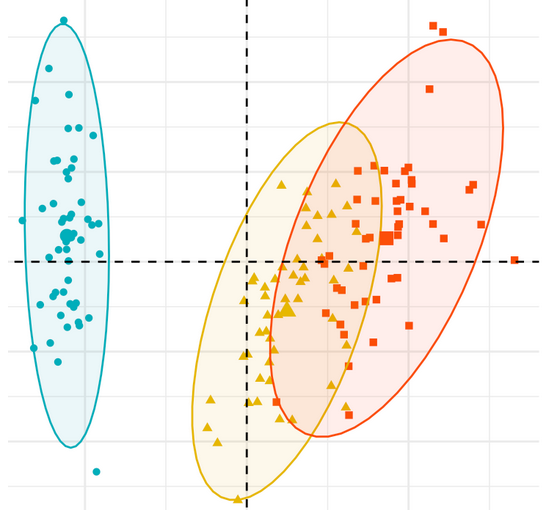
\includegraphics[height=8cm]{logos/accueil.png}
\end{center}

\vspace{10mm}

\textbf{Mémoire présenté et soutenu à $lieu$}

\textbf{En $date_jma$, par}

\Large {\color{Prune} \textbf{$prenom$ $nom$}}

\vspace{15mm}

\flushleft \normalsize \textbf{Composition du jury~:}
\bigskip

\scriptsize
\arrayrulecolor{Prune}
\begin{tabular}{|p{4cm}l}
\textbf{$jur1_nom$} &  $jur1_qualite$\\
$jur1_titre$ & \\
\textbf{$jur2_nom$} &  $jur2_qualite$\\
$jur2_titre$ & \\
% \textbf{$jur3_nom$} &  $jur3_qualite$\\
% $jur3_titre$ & \\
% \textbf{$jur4_nom$} &  $jur4_qualite$\\
% $jur4_titre$ & \\
% \textbf{$jur5_nom$} &  $jur5_qualite$\\
% $jur5_titre$ & \\
% \textbf{$jur6_nom$} &  $jur6_qualite$\\
% $jur6_titre$ & \\
\end{tabular}

% \begin{tabular}{p{8cm}l}
% & \\
% \textbf{$jur7_nom$} &  $jur7_qualite$\\
% $jur7_titre$ & \\
% \textbf{$jur8_nom$} &  $jur8_qualite$\\
% $jur8_titre$ & \\
% \textbf{$jur9_nom$} &  $jur9_qualite$\\
% $jur9_titre$ & \\
% \end{tabular}

\end{titlepage}

\addamargin % this add the margin back

\frontmatter % this stuff will be roman-numbered
\pagestyle{empty} % this removes page numbers from the frontmatter

$if(acknowledgements)$
  \begin{acknowledgements}
    $acknowledgements$
  \end{acknowledgements}
$endif$

$if(abstract)$
  \begin{abstract}
    $abstract$
  \end{abstract}
$endif$

% $if(preface)$
%   \begin{preface}
%     $preface$
%   \end{preface}
% $endif$

$if(toc)$
  \hypersetup{linkcolor=$if(toccolor)$$toccolor$$else$black$endif$}
  \setcounter{secnumdepth}{$toc-depth$}
  \setcounter{tocdepth}{$toc-depth$}
  \tableofcontents
$endif$

$if(lot)$
  \listoftables
$endif$

$if(lof)$
  \listoffigures
$endif$

$if(dedication)$
  \begin{dedication}
    $dedication$
  \end{dedication}
$endif$

\mainmatter % here the regular arabic numbering starts
\pagestyle{fancyplain} % turns page numbering back on

$body$


% 4eme de couverture
% \ifthispageodd{}{\newpage\thispagestyle{empty}\null}
% Use the next command with TeX Live version ≥ 2020
%\Ifthispageodd{}{\newpage\thispagestyle{empty}\null}
\newpage
\thispagestyle{empty}
\newgeometry{top=1.5cm, bottom=1.25cm, left=2cm, right=2cm}
\fontfamily{rm}\selectfont

\lhead{}
\rhead{}
\rfoot{}
\cfoot{}
\lfoot{}

\noindent
%*****************************************************
%***** LOGO DE L'EDMH *********
%*****************************************************
% \includegraphics[height=4.5cm]{$logo_ecole_doctotrale$}
% \vspace{1cm}
%*****************************************************

\begin{mdframed}[linecolor=Prune,linewidth=1]
\vspace{-.25cm}
\paragraph*{Titre~:} $titre_francais$
\begin{small}
\vspace{-.25cm}
\paragraph*{Mots clés~:} $mots_clefs_francais$

\vspace{-.5cm}
\begin{multicols}{2}
\paragraph*{Résumé~:} $resume_francais$
\end{multicols}
\end{small}
\end{mdframed}

\begin{mdframed}[linecolor=Prune,linewidth=1]
\vspace{-.25cm}
\paragraph*{Title:} $titre_anglais$

\begin{small}
\vspace{-.25cm}
\paragraph*{Keywords:} $mots_clefs_anglais$

\vspace{-.5cm}
\begin{multicols}{2}
\paragraph*{Abstract:} $resume_anglais$
\end{multicols}
\end{small}
\end{mdframed}


\vfill
\fontfamily{fvs}\fontseries{m}\selectfont
\noindent\begin{tabular}{p{14cm}}
\multirow{3}{16cm}[+0mm]{\small {\color{Prune} {\bf Université Paris-Saclay}\\
{\scriptsize Espace Technologique / Immeuble Discovery}\\
{\scriptsize  Route de l’Orme aux Merisiers RD 128 / 91190 Saint-Aubin, France}}}\\\mbox{}
\end{tabular}


% Index?

\end{document}
